

\section{Constraint formulation}\label{se:model}
Compared with other formulations, the features of our model are as follows.
First, we evaluate the allocation and scheduling strategy for a certain number of iterations, instead of once execution of every task. This allows a more accurate system evaluation. Second, additional to the deadline for every task, we put forward the concept of latest response time between two tasks, to meet the requirements of time-critical systems. Third, we consider fine-grained communication in the case of contentions. Finally, besides energy consumption and performance optimization, we also consider to minimize the probability of contention caused by communication from different resources in a communication network, which is evaluated by the overlapped area between two communication paths. 

%The hardware architecture considered here is a general framework, e.g., MPSoCs or NoCs. 
%%The performance is still evaluated with makespan, which is the duration of the executing of an application. 
%We assume that communication does not occupy computation resources, except for setup efforts.
%The channel for communication may consist of multiple links and nodes. Multiple data transfer may happen at the same time, or cannot overlapped, which is decided by the architecture.

First, we introduce the variables and constants used in our formulation in Table \ref{tab:var}, to present the constraints in allocating and scheduling issues.
\begin{table}[t]\caption{Constants and Variables \label{tab:var}}
\centering\small
\begin{tabular}{l l}\hline
Item & explanation\\\hline$bw$ & the bandwidth of a link \\
$\tau$& the time  of transferring a unit with unit distance\\
$\tau'$& the time  of transferring a unit through a node\\
$\epsilon$ & the energy of transferring a unit with unit distance\\
$\epsilon'$ & the energy of transferring a unit through a node\\
$a_i$ & the amount of computation for task $t_i$ \\
$c_{ij}$ & the amount of data to be transferred from task $t_i$ to $t_j$\\
%$q_i$ & the required size for data storage of $t_i$\\ 
$dl_{ij}$ & maximal time allowed between executing task $t_i$ and $t_j$\\
$\rho_k$ & processing speed of  $p_k$\\
$\omega_k$  & the memory limit for $p_k$ \\
%$\eta$ & the cost of communication setup \\
$\gamma_{{i_1}{j_1}{i_2}{j_2}}$ & the number of shared transmission path exists from $p_{i_1}$ to $p_{j_1}$ and from $p_{i_2}$ to $p_{j_2}$\\
$\xi$ & the time bound for simultaneous communication \\
$N$ & the number of iterations for all the tasks\\\hline
$m_{ik}$ & task $t_i$ is mapped to  $p_k$ \\
$n_{ij}$ & task $t_j$ is executed next to $t_i$ on the same processor\\
$s_i$  & the start time of executing task $t_i$ \\
$f_i$& the end time of executing task $t_i$ \\
$se_{ij}$ & the start time of data transfer from $t_i$ to $t_j$\\
$fe_{ij}$ & the finish time of data transfer from $t_i$ to $t_j$\\
%$ss_i$  & the start time of data transfer for task $t_i$ \\
%$fs_i$& the end time of data transfer for task $t_i$ \\
%$sr_i$  & the start time of receiving data for task $t_i$ \\
%$fr_i$& the end time of receiving data for task $t_i$ \\
$d_{ij}$ & task $t_j$ depends on the output of $t_i$\\
$o_{ij}$ & task $t_i$ needs to send data to its successor\\
$D_{ij}$ & distance between $p_i$ and $p_j$\\
$P_{ij}$ & the contention probability of data transfer from two tasks\\
\hline
\end{tabular}
\end{table}

%\begin{table}[htp]\caption{Constants\label{tab:con}}
%\centering
%\begin{tabular}{ll}\hline
%Item & explanation\\\hline
%$bw$ & the bandwidth of a link \\
%$\tau$& the time  of transferring a unit with unit distance\\
%$\tau'$& the time  of transferring a unit through a node\\
%$\epsilon$ & the energy of transferring a unit with unit distance\\
%$\epsilon'$ & the energy of transferring a unit through a node\\
%$a_i$ & the amount of computation for task $t_i$ \\
%$c_{ij}$ & the amount of data to be transferred from task $t_i$ to $t_j$\\
%%$q_i$ & the required size for data storage of $t_i$\\ 
%$dl_{ij}$ & maximal time allowed between executing task $t_i$ and $t_j$\\
%$\rho_k$ & processing speed of  $p_k$\\
%$\omega_k$  & the memory limit for $p_k$ \\
%%$\eta$ & the cost of communication setup \\
%$\gamma_{{i_1}{j_1}{i_2}{j_2}}$ & the number of shared transmission path exists from $p_{i_1}$ to $p_{j_1}$ and from $p_{i_2}$ to $p_{j_2}$\\
%$\xi$ & the time bound for simultaneous communication \\
%$N$ & the number of iterations for all the tasks\\
%\hline
%\end{tabular}
%\end{table}

In Table \ref{tab:con} can be computed according to the positions of processors. Given processors $p_{i_1}$, $p_{j_1}$, $p_{i_2}$ and $p_{j_2}$, let $(x_i,y_i)$ be the location of $p_i$. We have 
\begin{small}
 $$oX'=(x_{j1}-x_{i_1})+(x_{j2}-x_{i_2})-(max\{x_{j_1},x_{j_2}\}-min\{x_{i_1},x_{i_2}\})$$
 $$oY'=(y_{j1}-y_{i_1})+(y_{j2}-y_{i_2})-(max\{y_{j_1},y_{j_2}\}-min\{y_{i_1},y_{i_2}\}).$$
\end{small}
Let $oX=max\{oX',0\}$, and $oY=max\{oY',0\}$. We have $\gamma_{{i_1}{j_1}{i_2}{j_2}}=oX+oY$.  

\subsection{Constraints}
The constraints can be divided into two types: static mapping and dynamic behaviors. For behavior constraints, they consist of computation and communication behaviors. 

\subsubsection{Static constraints}
\begin{equation}\label{eq:map}
\sum^{|P|}_{k=1} m_{ik} =1
\end{equation}
\begin{equation}\label{eq:cap}
\sum^{|T|}_{i=1} m_{ik} \cdot q_i \leq \omega_k
\end{equation}
\begin{equation}\label{eq:neighbor}
n_{ij} + n_{ji} \leq 1 \wedge (n_{ij}\wedge n_{jl} \rightarrow \neg n_{il}), ~~n_{ij}\leq m_{ik}\cdot m_{jk'}
\end{equation}
\begin{equation}\label{eq:aux}
d_{ij}\wedge m_{ik}\wedge m_{jk'}\wedge (k\neq k') \rightarrow o_{ij}, ~~o_{ij}\rightarrow d_{ij}
\end{equation}
Constraint \ref{eq:map} requires that one task can only be mapped to one processor.
Constraint \ref{eq:cap} specifies that the capacity of a processor cannot be violated.
Constraint \ref{eq:neighbor} explains that the next-door execution relation is not transitive and reflexive.
Constraint \ref{eq:aux} reasons the case with communication cost.

\subsection{Dynamic behaviors}
First, we present precedence relation for computation and communication.
\begin{equation}\label{eq:response}
s^v_j-s^u_i\leq dl_{ij}
\end{equation}
\begin{equation}\label{eq:datar}
\sum^{|T|}_{j=1}d_{ji}>0 \rightarrow fe^u_{ji} \leq s^u_i
\end{equation}
\begin{equation}\label{eq:datas}
f^u_i\leq se^u_{ij}
\end{equation}
\begin{equation}\label{eq:next}
n_{ij} \rightarrow f^u_i \leq s^v_j \textrm{, for~} u\leq v
\end{equation}
\begin{equation}\label{eq:period}
m_{ik}\wedge m_{jk}  \rightarrow f^u_j \leq s^v_i \textrm{, for~} u<v
\end{equation}
Constraint \ref{eq:response} specifies that  the response time between certain tasks should less than the defined limitation.
Constraint \ref{eq:datar} requires that the start of executing $t_i$ should wait for data being transferred, except for the one without any predecessor.
Constraint \ref{eq:datas} specifies that the start of data transfer has to wait for the finish of task execution.
Constraint \ref{eq:next} requires that for two tasks scheduled next to each other in the same processor, the start of the latter should wait for the finish of the former, where $u\leq v$.
Constraint \ref{eq:period} explains that  the execution of task in later iteration $v$ should not be earlier than any other tasks executed on the same processor in an earlier iteration $u$, where $u<v$.

Next, we present constraints to avoid overlapped computation and communication. 

\begin{equation}\label{eq:overlap}
m_{ik}\wedge m_{jk} \rightarrow s^u_j\geq f^u_i \vee s^u_i\geq  f^u_j
\end{equation}
%\begin{equation}\label{eq:commlap}
%m_{ik}\wedge m_{lk}\rightarrow se^u_{ij}\geq fe^u_{lr} \vee se^u_{lr}\geq  fe^u_{ij}
%\end{equation}
\begin{equation}\label{eq:samesource}
\gamma_{{i}{j}{i}{r}} \rightarrow se^u_{ij}-se^u_{ir}\geq \xi
\end{equation}
\begin{equation}\label{eq:linklap}
\gamma_{{i}{j}{l}{r}}\wedge abs(f_{i}-f_{l})\leq \xi \rightarrow se^u_{ij}\geq fe^u_{lr} \vee se^u_{lr}\geq  fe^u_{ij}
\end{equation}

Constraint \ref{eq:overlap} specifies that two tasks executed on the same processor cannot be overlapped. 
%Constraint \ref{eq:commlap} explains  two communications from the same source cannot overlap.
Constraint \ref{eq:samesource} says that data transfer sharing same links from the same source cannot be triggered simultaneously. 
Constraint \ref{eq:linklap} says that two communication with shared resource cannot overlap, if their tasks finish execution almost at the same time. This constraint aims to allow the following case shown in Figure~\ref{fig:overlap}. A short communication path from $p_2$ to $p_3$ is overlapped by a long communication path from $p_0$ to $p_3$. But the communication of the short path can be finished before the long transmission arrives the shared path. 
%\item before receiving, a successor has wait for the finish of data transfer from its predecessor 
%\begin{equation}\label{eq:dependency}
%d_{ij}\wedge m_{ik}\wedge m_{jk'}\rightarrow fs^u_i \leq sr^u_j
%\end{equation}
\begin{figure}[h]
\centering
 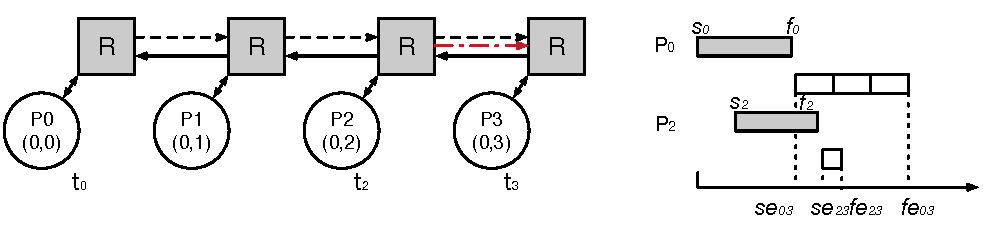
\includegraphics[width=0.85\columnwidth]{figures/overlap.pdf}% \vspace{-4.5mm}
  \caption{An example with communication overlap.}
 \label{fig:overlap}
% \vspace{-3mm}
 \end{figure}

Next we present quantitative relation for the variables on computation and communication.

\begin{equation}\label{eq:comp}
f^u_i = s^u_i + a_i/(\sum^{|P|}_{k=1} m_{ik}\cdot \rho_k)
\end{equation}
\begin{equation}\label{eq:comm}
fe^u_{ij} \geq se^u_{ij} +  o_{ij}\cdot(c_{ij} \cdot\tau\cdot  D_{ij}/bw+\tau'\cdot (D_{ij}+1))
\end{equation}
Constraint \ref{eq:comp} presents task execution relation.
Constraint \ref{eq:comm} shows that the finish of a data transfer considers the distance of the destination%two processors $p_k$ and $p_{k'}$
where $D_{ij}$ is the distance from the located processor of $t_i$ to the target processor. 

%\noindent\textbf{Discussion.} 
%The constraints listed above are flexible. For example, Constraint \ref{eq:period} can be relaxed such that a task can be executed several times before the next scheduled.

%As these constraints are for a general framework, we can adjust it according to specific architectures, especially for communication issues. For example, if the architecture allows multiple communication simultaneously,  Equation \ref{eq:commlap} can be relaxed.
%
%The communication link for different architectures may be quite different. For an MPSoC with buses connected to processors, there is not intermediate node or link between two processors. However, for an NoC, the situation is quite different, where the communication between two processors is fulfilled through links for transmission and switches for router.
%%Compared with general MPSoCs, the communication cost in NoC is more complex to evaluate, which consider the number of links and switches between two communicated processors.
%
%We consider 2D-mesh NoC, where the effort for communication can be computed according to the distance between two processors $p_i$ and $p_j$, where $(x_i,y_i)$ is the location of $p_i$\cite{huang2011energy}:
%\begin{equation}\label{eq:dis}
%D_{ij}=abs(x_i-x_j)+abs(y_i-y_j)
%\end{equation}

\subsection{Optimization objectives}

With the defined variables, the makespan of  executing an application within $N$ iterations is 
\begin{equation}\label{eq:makespan}
{\cal{M}}=max\{f^N_i\}
\end{equation}
However, energy consumption includes cost for computation $E_p$ and communication $E_m$. For computation, we distinguish different status in a processor and accumulate the total cost. For communication, we consider the cost for routing and data transfer. In a NoC network, the number of available processors may be larger than that of tasks. We use $P'=\{p_k\;| \sum^{|T|}_{i=1} m_{ik}>0\}$ to denote the set of occupied processors. 

A processor may switch between dynamic, static and sleep modes, to save energy consumption. If the idle time is less than $t_{o}$, the processor will not switch into sleep mode. Otherwise, a time penalty $t_\Delta$  for switching into and out of sleep is considered, together with an energy penalty $\epsilon_\Delta$.
%We ignore power leakage, for we take computation load balance as one of optimization goals, which can keep the chip in a relative steady temperature. 
The execution duration of every iteration in a processor may be different, thus the cost should differ. Let $t_h$ be head of scheduled task in a processor $p_k$ in every iteration, where the constraint  $\sum^{|T|}_{j=1} m_{jk}-1=\sum^{|T|}_{j=1} q_{k_{hj}}$ holds. The duration ${\mathcal{D}}^u_{k}$ for processor $p_k$ in iteration $u$ is
\begin{equation}\label{eq:duration}
{\mathcal{D}}^u_{k} =\left\{
\begin{array}{ll}
\tau^{u+1}_h -\tau^u_h & u<N\\
{\mathcal{M}} - \tau^N_h & u=N
\end{array}
\right.
\end{equation}
Let $t_l$ be the tail of scheduled task in $p_k$, with $\sum^{|T|}_{i=1} q_{k_{li}}+1=m_{lk}$.
Then the spare time ${\mathcal{S}}^u_{k_{ij}} $for a processor $p_k$ executing two successive tasks $t_i$ and $t_j$ in iteration $u$ can be computed as follows:
\begin{equation}\label{eq:spare}
{\mathcal{S}}^u_{k_{ij}} =\left\{
\begin{array}{ll}
0 & \gamma_{k_{ij}}=0\wedge i\neq l\\
\tau^u_j-e^u_i & \gamma_{k_{ij}}=1 \wedge i\neq l\\
{\mathcal{D}}^u_k-e^u_i & i=l
\end{array}\right.
\end{equation}

Let ${\mathcal{P}}_{d_k}$, ${\mathcal{P}}_{i_k}$ and ${\mathcal{P}}_{s_k}$ be the rate of dynamic, static (idle) and sleep power consumption of processor $p_k$, respectively. The costs for dynamic ($E_d$), static and sleep ($E_{is}$) are calculated as follows:
 \begin{equation}
E_d = N\cdot \sum^{|P'|}_{k=1}({\mathcal{P}}_{d_k}\cdot \sum^{|T|}_{i=1}  \theta_i \cdot m_{ik})
\end{equation}%\vspace{-10pt}
\begin{equation}\label{eq:ei}
E_{is} =\sum^N_{u=1}\sum^{|P'|}_{k=1}\sum^{|T|}_{i,j=1}\left\{
\begin{array}{ll}
{\mathcal{P}}_{s_k}\!\!\cdot ({\mathcal{S}}^u_{k_{ij}}-t_\Delta) + \epsilon_\Delta & {\mathcal{S}}^u_{k_{ij}} \!\!\geq t_{o} \\
 {\mathcal{P}}_{i_k}\!\!\cdot {\mathcal{S}}^u_{k_{ij}} &0 \leq {\mathcal{S}}^u_{k_{ij}}\!\! <t_{o} %\\
 %0 & ~~{\mathcal{S}}^u_{k_{ij}}=0
\end{array}
\right.
	%E_i= \sum^{|P|}_{k=1} (Ri_k \cdot ({\cal{M}}- N\cdot \sum^{|T|}_{i=1}  \theta_i \cdot m_{ik} ) )
\end{equation}%\vspace{-14pt}




The energy cost for communication is evaluated according to the amount of data and the distance of the transmission. 
\begin{equation}\label{eq:ecomm}
E_m = N\cdot  \sum^{|P'|}_{k,k'=1} \sum^{|T|}_{i,j=1} c_{ij}\cdot o_{ij}\cdot m_{ik}\cdot m_{jk'}\cdot (\epsilon\cdot  D_{kk'}+ \epsilon'\cdot (D_{kk'}+1))
\end{equation}

Addition to the energy and makespan optimization, we also expect that the probability of communication contention is reduced. As data transfer occurs in the end of task execution, we consider the potential contention when two tasks at various processors finish execution almost simultaneously (their difference is less than a limited time bound. The probability is evaluated according to the overlapped path between two communication paths in a communication network. Suppose two paths are from processor $i_1$ to $j_1$, and $i_2$ to $j_2$ respectively.  
%Let $oX$ and $oY$ be the overlapped width and length of the two paths. That is
%\begin{small}
% $$oX=(x_{j1}-x_{i_1})+(x_{j2}-x_{i_2})-(max\{x_{j_1},x_{j_2}\}-min\{x_{i_1},x_{i_2}\})$$
% $$oY=(y_{j1}-y_{i_1})+(y_{j2}-y_{i_2})-(max\{y_{j_1},y_{j_2}\}-min\{y_{i_1},y_{i_2}\}).$$
%\end{small}
% If $oX\leq 0$ or $oY\leq 0$, there is no contention. Therefore, we have $oX=max\{oX,0\}$, and $oY=max\{oY,0\}$. 
% Let the areas of the two paths be $S_1=abs((x_{i_1}-x_{j_1})\cdot (y_{i_1}-y_{j_1}))$ and  $S_2=abs((x_{i_2}-x_{j_2})\cdot (y_{i_2}-y_{j_2}))$ respectively. 
The contention probability of two paths is 
\begin{equation}
%p_c({i_1},{j_1},{i_2},{j_2})=oX\cdot oY/(S_1+S_2)
p_c({i_1},{j_1},{i_2},{j_2})=(oX+ oY)/(D_{{i_1}{j_1}}\cdot D_{{i_2}{j_2}})
\end{equation}

For any two tasks $t_{i_1}$ and $t_{i_2}$, let ${\mathcal{T}_{i}}$ be the set of successors of task $t_i$. Then the measure of contention of communication is 
\begin{equation}\label{eq:submeasure}
P_{{i_1}{i_2}}=\sum_{j_1\in {\mathcal{T}_{i_1}}, j_2 \in {\mathcal{T}_{i_2}}}(abs(f^u_{i_1} -f^v_{i_2})\leq \xi)\cdot o_{{i_1}{j_1}}\cdot o_{{i_2}{j_2}}\cdot p_c(k_{i_1},k_{j_1},k_{i_2},k_{j_2})
\end{equation}
%However, data transmission is fulfilled by bus in an MPSoC, we have 
%\begin{equation}
%P_{{i_1}{i_2}=}(abs(f^u_{i_1} -f^v_{i_2})\leq \xi)
%\end{equation}
According Equation \ref{eq:submeasure}, the measure for a mapping and scheduling strategy is 
\begin{equation}
P_c=\sum^{|T|}_{i,j=1} P_{ij}
\end{equation}
We apply the average contention probability to evaluate the quality of the allocation strategy, which is denoted by
\begin{equation}
\bar{P_c}=\sum^{|T|}_{i,j=1}abs(P_{ij}-P_c/(|T|\cdot N))
\end{equation} 
Based on the discussion above, we can have three objectives to be optimized: makespan, total amount of energy cost, and contention:
\begin{equation}\label{eq:makespan}
minimize({\cal{M}})
\end{equation}
\begin{equation}\label{eq:energy}
minimize(E_{pd} +E_{is}+ E_m)
\end{equation}
\begin{equation}\label{eq:contention}
minimize(\bar{P_c})
\end{equation}
\noindent\textbf{Discussion.} 
Constraint \ref{eq:linklap} and Objective \ref{eq:contention} are complementary. Constraint \ref{eq:linklap} considers the temporal relation of contention, and separates the potential overlapped communication mandatory to avoid contention. Objective \ref{eq:contention} focus on spatial contention and tries to minimize the overlapped communication paths. 
%For an NoC, workload balance is not the main concern, for the number of available processors may be greater than that of tasks.


